\section{Luminosity Functions} \label{Sec: Luminosity Functions}
\subsection{Vmax} \label{Sec: Vmax}
To estimate the LF from our data, we utilise the $1/V_{max}$ method \citep{schmidt_space_1968}. The $1/V_{max}$ method is well-suited for surveys like ZFOURGE, as it does not assume any specific shape for the LF and can easily accommodate galaxies observed across varying depths. It accounts for the maximum observable volume of each galaxy and is given by equation \ref{EQ: 1/Vmax}:

\begin{equation} \label{EQ: 1/Vmax}
    \phi(L,z) = \frac{1}{\Delta \log L}\sum_{i=1}^N \frac{1}{V_{max,i}}
\end{equation}

Where $V_{max}$ represents the maximum co-moving volume of the $i$-th source and $\Delta$ log(L) is the width of the luminosity bin. In practice, to observe the evolution of the LF through cosmic time, the maximum observable volume ($V_{max}$) is calculated for each redshift bin where the upper and lower bounds of the redshift bin limit the volume. Additionally, redshift bins are split into luminosity bins to observe the number density evolution across the different classes of luminosity such as LIRGs (10$^{11} < L_{IR} < 10^{12}\ L_{\odot}$) and ULIRGs ($L_{IR} > 10^{12}\ L_{\odot}$). $V_{max}$ of each galaxy is calculated by taking the maximum comoving volume of the redshift bin the galaxy resides in and subtracting the comoving volume at the beginning of the redshift bin (equation \ref{EQ: Vmax}). We account for the survey area of ZFOURGE (0.1111 degrees$^2$), which normalises the volume probed across the sky (41,253 degrees$^2$). 

\begin{figure*}
    \centering
    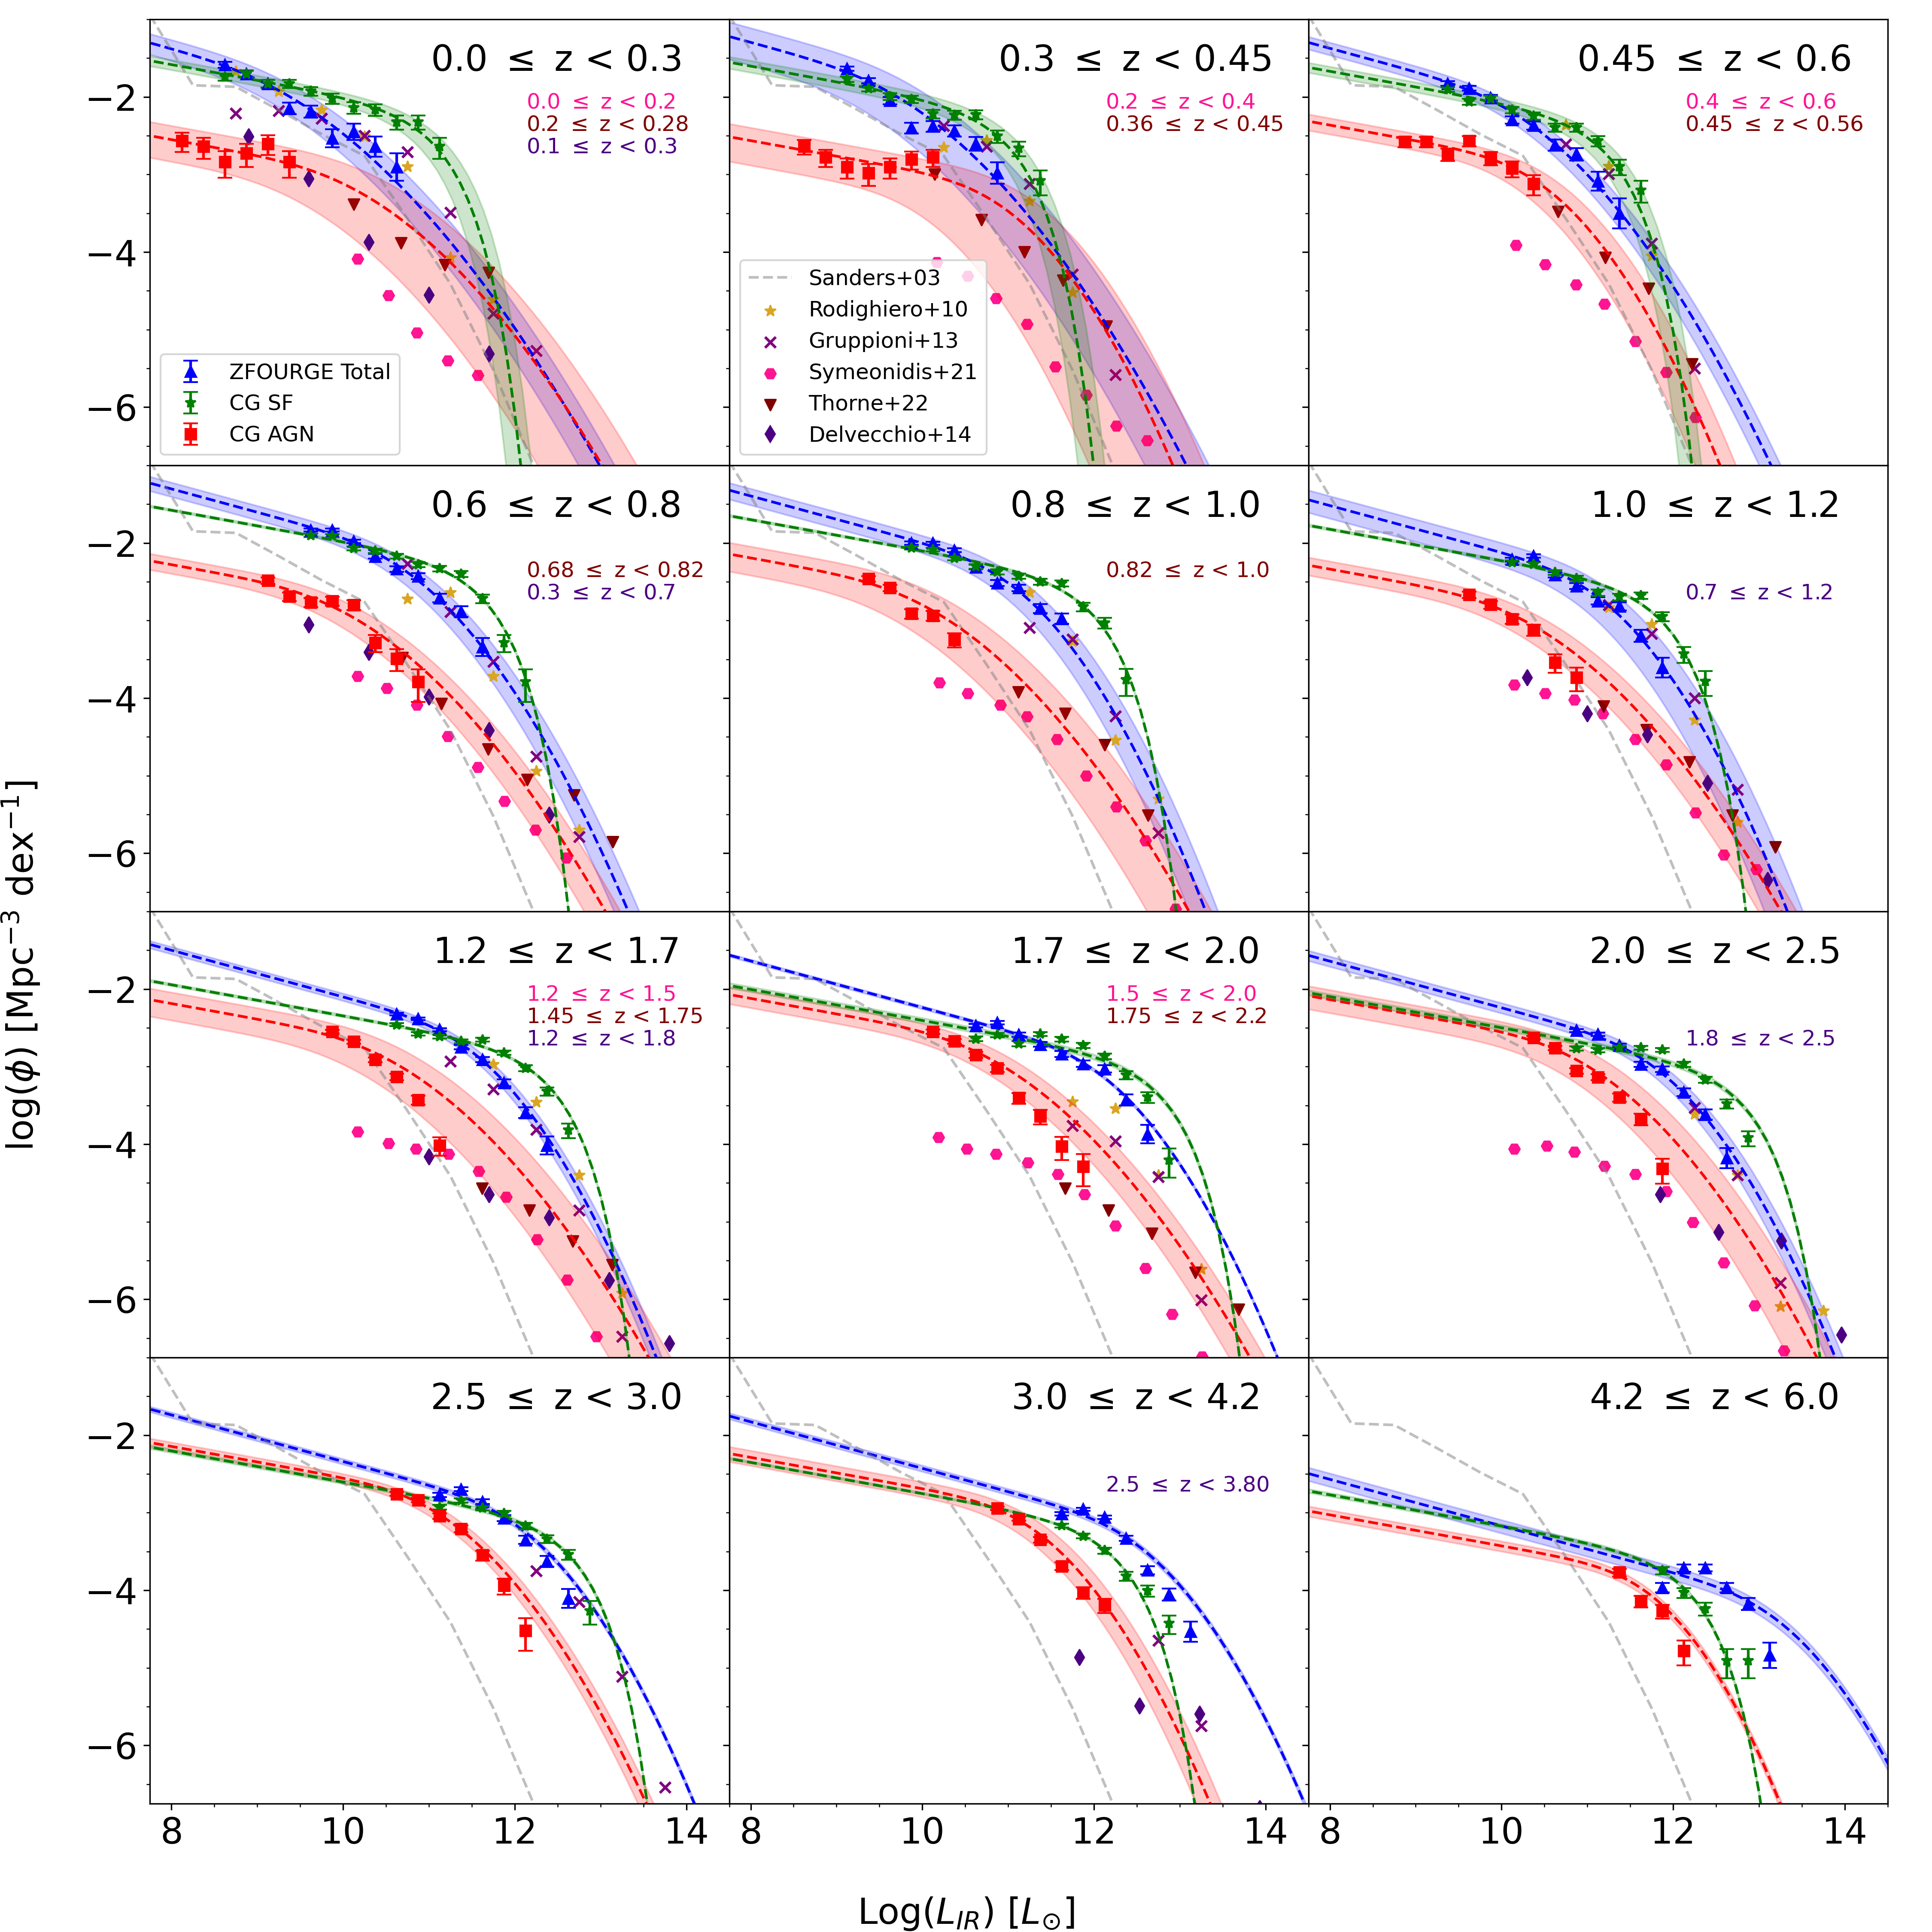
\includegraphics[width=\textwidth]{Figures/LF.png}
    \caption{The luminosity functions of major galaxy populations in ZFOURGE and CIGALE calculated using the Vmax method. The dark blue triangles present the ZFOURGE bolometric IR (8-1000$\mu$m) LF. The CIGALE SF and AGN LFs are the green stars and red squares, respectively. The blue and red dashed lines show the best fit Saunders function \citep{saunders_60-mum_1990} to the ZFOURGE total and CIGALE AGN LF, respectively. The green dashed line shows the best-fit Schechter function \citep{schechter_analytic_1976} to the CIGALE SF LF. The shaded regions represent the $1\sigma$ functional fit errors. The luminosity completeness limit of each redshift bin is where we stop displaying fainter $\phi$ values. Where possible, comparable literature results are also shown. The local \cite{sanders_iras_2003} luminosity function is shown across all redshift bins as the grey dashed line. \cite{rodighiero_mid-_2010} is shown as gold filled stars from $0 < z < 2.5$, \cite{gruppioni_herschel_2013} as purple crosses from $0 < z < 4.2$, \cite{symeonidis_agn_2021} AGN as pink hexagons, \cite{thorne_deep_2022} AGN as maroon upside-down triangles, \cite{delvecchio_tracing_2014} AGN as indigo diamonds. Differing redshift bins are colour-labelled accordingly. Our ZFOURGE total results are consistent with various sources across redshift bins in the literature \citep{caputi_infrared_2007, huang_local_2007, fu_decomposing_2010}}
    \label{Fig: Bolometric IR LF}
\end{figure*}

\begin{equation}
    \label{EQ: Vmax}
    V_{max,i} = \frac{4}{3} \pi \left(D_{max}^3 - D_{min}^3\right) \times \frac{A}{41,253}
\end{equation}

We calculate the maximum ($D_{max}$) and minimum ($D_{min}$) comoving distances for all sources within each redshift bin using the \texttt{FlatLambdaCDM} model from the \texttt{Astropy} Python package \citep{astropy_collaboration_astropy_2022}. These calculations are performed for sources above the luminosity-completeness limits (coloured sources of figure \ref{Fig: ZF Lum vs z}). We limit each luminosity bin to a minimum of five sources, or else the luminosity bin is discarded. 

Sources with $D_{max}$ values that do not extend to the end of the redshift bin are removed to avoid bias from sources incompletely sampled within the bin. Different redshift bins have different volumes, and each luminosity bin has a different number density $\phi$. $D_{min}$ and $D_{max}$ are the comoving distances at the beginning and end of the redshift bin, respectively, for all galaxies. The relative LF number density $1\sigma$ error values are calculated with:

\begin{equation} \label{EQ: Vmax Error}
    \phi(L,z) = \frac{1}{\Delta \log L}\sqrt{\sum_i \frac{1}{V_{max}^2}}
\end{equation}

\begin{landscape}
    \begin{table*}
    \begin{center}
    \caption{ZFOURGE bolometric IR (8-1000$\mu$m) LF $\phi$ values.}
    \label{Tab: ZF LF}
    \begin{tabular}{@{}ccccccc@{}}
        \toprule
        $\log_{10}(L_{IR}/L_{\odot})$ & 0.00 $\leq z <$ 0.30 & 0.30 $\leq z <$ 0.45 & 0.45 $\leq z <$ 0.60 & 0.60 $\leq z <$ 0.80 & 0.80 $\leq z <$ 1.00 & 1.00 $\leq z <$ 1.20 \\
        \hline
         8.50 --  8.75 & -1.58 $\pm$ 0.04 & - & - & - & - & - \\
         8.75 --  9.00 & -1.70 $\pm$ 0.04 & - & - & - & - & - \\
         9.00 --  9.25 & -1.83 $\pm$ 0.05 & -1.64 $\pm$ 0.03 & - & - & - & - \\
         9.25 --  9.50 & -2.15 $\pm$ 0.07 & -1.79 $\pm$ 0.03 & -1.83 $\pm$ 0.03 & - & - & - \\
         9.50 --  9.75 & -2.19 $\pm$ 0.08 & -2.05 $\pm$ 0.05 & -1.89 $\pm$ 0.03 & -1.83 $\pm$ 0.02 & - & - \\
         9.75 -- 10.00 & -2.54 $\pm$ 0.12 & -2.40 $\pm$ 0.07 & -2.01 $\pm$ 0.03 & -1.83 $\pm$ 0.02 & -2.00 $\pm$ 0.02 & - \\
        10.00 -- 10.25 & -2.45 $\pm$ 0.11 & -2.38 $\pm$ 0.07 & -2.30 $\pm$ 0.05 & -1.98 $\pm$ 0.02 & -2.00 $\pm$ 0.02 & -2.21 $\pm$ 0.03 \\
        10.25 -- 10.50 & -2.64 $\pm$ 0.13 & -2.44 $\pm$ 0.07 & -2.37 $\pm$ 0.05 & -2.17 $\pm$ 0.03 & -2.09 $\pm$ 0.02 & -2.17 $\pm$ 0.02 \\
        10.50 -- 10.75 & -2.90 $\pm$ 0.18 & -2.60 $\pm$ 0.09 & -2.62 $\pm$ 0.07 & -2.34 $\pm$ 0.04 & -2.31 $\pm$ 0.03 & -2.41 $\pm$ 0.03 \\
        10.75 -- 11.00 & -                & -2.98 $\pm$ 0.14 & -2.74 $\pm$ 0.08 & -2.43 $\pm$ 0.04 & -2.52 $\pm$ 0.04 & -2.56 $\pm$ 0.04 \\
        11.00 -- 11.25 & -                & -                & -3.09 $\pm$ 0.12 & -2.71 $\pm$ 0.06 & -2.58 $\pm$ 0.04 & -2.75 $\pm$ 0.05 \\
        11.25 -- 11.50 & -                & -                & -3.50 $\pm$ 0.19 & -2.89 $\pm$ 0.07 & -2.85 $\pm$ 0.06 & -2.82 $\pm$ 0.05 \\
        11.50 -- 11.75 & -                & -                & -                & -3.34 $\pm$ 0.12 & -2.98 $\pm$ 0.07 & -3.20 $\pm$ 0.08 \\
        11.75 -- 12.00 & -                & -                & -                & -                & -                & -3.61 $\pm$ 0.13 \\
        \hline
        $\log_{10}(L_{IR}/L_{\odot})$ & 1.20 $\leq z <$ 1.70 & 1.70 $\leq z <$ 2.00 & 2.00 $\leq z <$ 2.50 & 2.50 $\leq z <$ 3.00 & 3.00 $\leq z <$ 4.20 & 4.20 $\leq z <$ 6.00  \\
        \hline
        10.50 -- 10.75 & -2.33 $\pm$ 0.02 & -2.47 $\pm$ 0.02 & - & - & - & - \\
        10.75 -- 11.00 & -2.39 $\pm$ 0.02 & -2.43 $\pm$ 0.02 & -2.54 $\pm$ 0.02 & - & - & - \\
        11.00 -- 11.25 & -2.52 $\pm$ 0.02 & -2.59 $\pm$ 0.03 & -2.58 $\pm$ 0.02 & -2.77 $\pm$ 0.03 & - & - \\
        11.25 -- 11.50 & -2.75 $\pm$ 0.03 & -2.71 $\pm$ 0.03 & -2.73 $\pm$ 0.02 & -2.70 $\pm$ 0.02 & - & - \\
        11.50 -- 11.75 & -2.91 $\pm$ 0.03 & -2.84 $\pm$ 0.04 & -2.97 $\pm$ 0.03 & -2.86 $\pm$ 0.03 & -3.02 $\pm$ 0.02 & - \\
        11.75 -- 12.00 & -3.21 $\pm$ 0.05 & -2.96 $\pm$ 0.04 & -3.03 $\pm$ 0.03 & -3.07 $\pm$ 0.04 & -2.96 $\pm$ 0.02 & -3.97 $\pm$ 0.06 \\
        12.00 -- 12.25 & -3.59 $\pm$ 0.07 & -3.03 $\pm$ 0.05 & -3.33 $\pm$ 0.05 & -3.35 $\pm$ 0.05 & -3.06 $\pm$ 0.02 & -3.71 $\pm$ 0.05 \\
        12.25 -- 12.50 & -4.02 $\pm$ 0.12 & -3.43 $\pm$ 0.07 & -3.62 $\pm$ 0.07 & -3.63 $\pm$ 0.07 & -3.33 $\pm$ 0.03 & -3.71 $\pm$ 0.04 \\
        12.50 -- 12.75 & -                & -3.87 $\pm$ 0.12 & -4.18 $\pm$ 0.13 & -4.11 $\pm$ 0.12 & -3.74 $\pm$ 0.05 & -3.97 $\pm$ 0.06 \\
        12.75 -- 13.00 & -                & -                & -                & -                & -4.06 $\pm$ 0.08 & -4.18 $\pm$ 0.08 \\
        13.00 -- 13.25 & -                & -                & -                & -                & -4.53 $\pm$ 0.13 & -4.84 $\pm$ 0.16 \\
        \bottomrule
    \end{tabular}
    \end{center}
    \textbf{Note}: Luminosity bin $\phi$ values are centred.
    \end{table*}
\end{landscape}

\begin{landscape}
    \begin{table*}
    \begin{center}
    \caption{CIGALE AGN LF $\phi$ values.}
    \label{Tab: CG AGN LF}
    \begin{tabular}{@{}ccccccc@{}}
        \toprule
        $\log_{10}(L_{IR}/L_{\odot})$ & 0.00 $\leq z <$ 0.30 & 0.30 $\leq z <$ 0.45 & 0.45 $\leq z <$ 0.60 & 0.60 $\leq z <$ 0.80 & 0.80 $\leq z <$ 1.00 & 1.00 $\leq z <$ 1.20 \\
        \hline
         8.00 --  8.25 & -2.57 $\pm$ 0.12 & -                & -                & -                & -                & - \\
         8.25 --  8.50 & -2.64 $\pm$ 0.13 & -                & -                & -                & -                & - \\
         8.50 --  8.75 & -2.84 $\pm$ 0.16 & -2.64 $\pm$ 0.09 & -                & -                & -                & - \\
         8.75 --  9.00 & -2.74 $\pm$ 0.14 & -2.78 $\pm$ 0.11 & -2.58 $\pm$ 0.07 & -                & -                & - \\
         9.00 --  9.25 & -2.60 $\pm$ 0.13 & -2.90 $\pm$ 0.13 & -2.58 $\pm$ 0.07 & -2.48 $\pm$ 0.04 & -                & - \\
         9.25 --  9.50 & -2.84 $\pm$ 0.16 & -2.98 $\pm$ 0.14 & -2.74 $\pm$ 0.08 & -2.69 $\pm$ 0.05 & -2.46 $\pm$ 0.04 & - \\
         9.50 --  9.75 & -                & -2.90 $\pm$ 0.13 & -2.57 $\pm$ 0.07 & -2.76 $\pm$ 0.06 & -2.58 $\pm$ 0.04 & -2.67 $\pm$ 0.04 \\
         9.75 -- 10.00 & -                & -2.81 $\pm$ 0.11 & -2.79 $\pm$ 0.09 & -2.75 $\pm$ 0.06 & -2.91 $\pm$ 0.06 & -2.79 $\pm$ 0.05 \\
        10.00 -- 10.25 & -                & -2.78 $\pm$ 0.11 & -2.92 $\pm$ 0.10 & -2.80 $\pm$ 0.06 & -2.94 $\pm$ 0.06 & -2.98 $\pm$ 0.06 \\
        10.25 -- 10.50 & -                & -                & -3.12 $\pm$ 0.13 & -3.28 $\pm$ 0.11 & -3.25 $\pm$ 0.09 & -3.12 $\pm$ 0.07 \\
        10.50 -- 10.75 & -                & -                & -                & -3.49 $\pm$ 0.14 & -                & -3.54 $\pm$ 0.12 \\
        10.75 -- 11.00 & -                & -                & -                & -3.79 $\pm$ 0.19 & -                & -3.73 $\pm$ 0.14 \\
        \hline
        $\log_{10}(L_{IR}/L_{\odot})$ & 1.20 $\leq z <$ 1.70 & 1.70 $\leq z <$ 2.00 & 2.00 $\leq z <$ 2.50 & 2.50 $\leq z <$ 3.00 & 3.00 $\leq z <$ 4.20 & 4.20 $\leq z <$ 6.00  \\
        \hline
         9.75 -- 10.00 & -2.55 $\pm$ 0.02 & -                & -                & -                & -                & - \\
        10.00 -- 10.25 & -2.68 $\pm$ 0.02 & -2.55 $\pm$ 0.03 & -                & -                & -                & - \\
        10.25 -- 10.50 & -2.91 $\pm$ 0.03 & -2.67 $\pm$ 0.03 & -2.63 $\pm$ 0.02 & -                & -                & - \\
        10.50 -- 10.75 & -3.13 $\pm$ 0.04 & -2.85 $\pm$ 0.04 & -2.76 $\pm$ 0.03 & -2.76 $\pm$ 0.03 & -                & - \\
        10.75 -- 11.00 & -3.43 $\pm$ 0.06 & -3.02 $\pm$ 0.05 & -3.06 $\pm$ 0.04 & -2.84 $\pm$ 0.03 & -2.94 $\pm$ 0.02 & - \\
        11.00 -- 11.25 & -4.02 $\pm$ 0.12 & -3.40 $\pm$ 0.07 & -3.13 $\pm$ 0.04 & -3.04 $\pm$ 0.04 & -3.08 $\pm$ 0.02 & - \\
        11.25 -- 11.50 & -                & -3.64 $\pm$ 0.09 & -3.39 $\pm$ 0.05 & -3.21 $\pm$ 0.04 & -3.35 $\pm$ 0.03 & -3.77 $\pm$ 0.05 \\
        11.50 -- 11.75 & -                & -4.03 $\pm$ 0.14 & -3.68 $\pm$ 0.07 & -3.55 $\pm$ 0.06 & -3.69 $\pm$ 0.05 & -4.14 $\pm$ 0.07 \\
        11.75 -- 12.00 & -                & -4.29 $\pm$ 0.19 & -4.32 $\pm$ 0.15 & -3.94 $\pm$ 0.10 & -4.03 $\pm$ 0.07 & -4.27 $\pm$ 0.09 \\
        12.00 -- 12.25 & -                & -                & -                & -4.52 $\pm$ 0.19 & -4.19 $\pm$ 0.09 & -4.78 $\pm$ 0.15 \\
        \bottomrule
    \end{tabular}
    \end{center}
    \textbf{Note}: Luminosity bin $\phi$ values are centred.
    \end{table*}
\end{landscape}

\begin{landscape}
    \begin{table*}
    \begin{center}
    \caption{CIGALE SF LF $\phi$ values.}
    \label{Tab: CG SF LF}
    \begin{tabular}{@{}ccccccc@{}}
        \toprule
        $\log_{10}(L_{IR}/L_{\odot})$ & 0.00 $\leq z <$ 0.30 & 0.30 $\leq z <$ 0.45 & 0.45 $\leq z <$ 0.60 & 0.60 $\leq z <$ 0.80 & 0.80 $\leq z <$ 1.00 & 1.00 $\leq z <$ 1.20 \\
        \hline
         8.50 --  8.75 & -1.74 $\pm$ 0.05   & - & - & - & - & - \\
         8.75 --  9.00 & -1.70 $\pm$ 0.04   & - & - & - & - & - \\
         9.00 --  9.25 & -1.83 $\pm$ 0.05   & -1.77 $\pm$ 0.03  & - & - & - & - \\
         9.25 --  9.50 & -1.83 $\pm$ 0.05   & -1.89 $\pm$ 0.04  & -1.90 $\pm$ 0.03  & - & - & - \\
         9.50 --  9.75 & -1.93 $\pm$ 0.06   & -2.00 $\pm$ 0.04  & -2.06 $\pm$ 0.04  & -1.90 $\pm$ 0.02  & - & - \\
         9.75 -- 10.00 & -2.02 $\pm$ 0.06   & -2.03 $\pm$ 0.05  & -2.02 $\pm$ 0.04  & -1.91 $\pm$ 0.02  & -2.06 $\pm$ 0.02  & - \\
        10.00 -- 10.25 & -2.14 $\pm$ 0.07   & -2.22 $\pm$ 0.06  & -2.17 $\pm$ 0.04  & -2.07 $\pm$ 0.03  & -2.08 $\pm$ 0.02  & -2.25 $\pm$ 0.03 \\
        10.25 -- 10.50 & -2.16 $\pm$ 0.08   & -2.23 $\pm$ 0.06  & -2.25 $\pm$ 0.05  & -2.10 $\pm$ 0.03  & -2.20 $\pm$ 0.03  & -2.27 $\pm$ 0.03 \\
        10.50 -- 10.75 & -2.32 $\pm$ 0.09   & -2.23 $\pm$ 0.06  & -2.39 $\pm$ 0.05  & -2.17 $\pm$ 0.03  & -2.30 $\pm$ 0.03  & -2.38 $\pm$ 0.03 \\
        10.75 -- 11.00 & -2.32 $\pm$ 0.09   & -2.51 $\pm$ 0.08  & -2.39 $\pm$ 0.05  & -2.28 $\pm$ 0.03  & -2.37 $\pm$ 0.03  & -2.46 $\pm$ 0.03 \\
        11.00 -- 11.25 & -2.64 $\pm$ 0.13   & -2.66 $\pm$ 0.09  & -2.57 $\pm$ 0.07  & -2.33 $\pm$ 0.04  & -2.43 $\pm$ 0.04  & -2.64 $\pm$ 0.04 \\
        11.25 -- 11.50 & -                  & -3.08 $\pm$ 0.15  & -2.90 $\pm$ 0.10  & -2.40 $\pm$ 0.04  & -2.50 $\pm$ 0.04  & -2.70 $\pm$ 0.04 \\
        11.50 -- 11.75 & -                  & -                 & -3.20 $\pm$ 0.14  & -2.72 $\pm$ 0.06  & -2.52 $\pm$ 0.04  & -2.68 $\pm$ 0.04 \\
        11.75 -- 12.00 & -                  & -                 & -                 & -3.28 $\pm$ 0.11  & -2.82 $\pm$ 0.06  & -2.95 $\pm$ 0.06 \\
        12.00 -- 12.25 & -                  & -                 & -                 & -3.79 $\pm$ 0.19  & -3.03 $\pm$ 0.07  & -3.43 $\pm$ 0.10 \\
        12.25 -- 12.50 & -                  & -                 & -                 & -                 & -3.76 $\pm$ 0.16  & -3.78 $\pm$ 0.15 \\
        \hline
        $\log_{10}(L_{IR}/L_{\odot})$ & 1.20 $\leq z <$ 1.70 & 1.70 $\leq z <$ 2.00 & 2.00 $\leq z <$ 2.50 & 2.50 $\leq z <$ 3.00 & 3.00 $\leq z <$ 4.20 & 4.20 $\leq z <$ 6.00  \\
        \hline
        10.50 -- 10.75 & -2.46 $\pm$ 0.02   & -2.64 $\pm$ 0.03  & - & - & - & - \\
        10.75 -- 11.00 & -2.58 $\pm$ 0.02   & -2.59 $\pm$ 0.03  & -2.77 $\pm$ 0.03  & - & - & - \\
        11.00 -- 11.25 & -2.61 $\pm$ 0.02   & -2.70 $\pm$ 0.03  & -2.79 $\pm$ 0.03  & -2.93 $\pm$ 0.03  & - & - \\
        11.25 -- 11.50 & -2.67 $\pm$ 0.02   & -2.58 $\pm$ 0.03  & -2.76 $\pm$ 0.03  & -2.84 $\pm$ 0.03  & - & - \\
        11.50 -- 11.75 & -2.65 $\pm$ 0.02   & -2.65 $\pm$ 0.03  & -2.76 $\pm$ 0.03  & -2.94 $\pm$ 0.03  & -3.17 $\pm$ 0.03 & - \\
        11.75 -- 12.00 & -2.82 $\pm$ 0.03   & -2.73 $\pm$ 0.03  & -2.78 $\pm$ 0.03  & -3.01 $\pm$ 0.03  & -3.30 $\pm$ 0.03 & -3.74 $\pm$ 0.05 \\
        12.00 -- 12.25 & -3.02 $\pm$ 0.04   & -2.87 $\pm$ 0.04  & -2.97 $\pm$ 0.03  & -3.17 $\pm$ 0.04  & -3.49 $\pm$ 0.04 & -4.03 $\pm$ 0.06 \\
        12.25 -- 12.50 & -3.32 $\pm$ 0.05   & -3.11 $\pm$ 0.05  & -3.17 $\pm$ 0.04  & -3.34 $\pm$ 0.05  & -3.82 $\pm$ 0.06 & -4.24 $\pm$ 0.08 \\
        12.50 -- 12.75 & -3.82 $\pm$ 0.09   & -3.39 $\pm$ 0.07  & -3.48 $\pm$ 0.06  & -3.54 $\pm$ 0.06  & -4.01 $\pm$ 0.07 & -4.91 $\pm$ 0.18 \\
        12.75 -- 13.00 & -                  & -4.21 $\pm$ 0.18  & -3.92 $\pm$ 0.10  & -4.27 $\pm$ 0.14  & -4.43 $\pm$ 0.12 & -4.91 $\pm$ 0.18 \\
        \bottomrule
    \end{tabular}
    \end{center}
    \textbf{Note}: Luminosity bin $\phi$ values are centred.
    \end{table*}
\end{landscape}

\subsection{Fitting Functions}
We first construct the bolometric IR LF using the ZFOURGE dataset. Then, using CIGALE, we decompose the luminosity into contributions from SF regions and AGN, allowing us to investigate the evolution of these components separately.

To model LFs, one of the most widely used methods is the Schechter function \citep{schechter_analytic_1976}. This function is beneficial for describing the LF of galaxies because it can represent observed features, such as a power-law decline at the faint end and an exponential cutoff at the bright end. We employ the Schechter function to model the CIGALE SF LF as both \cite{fu_decomposing_2010} and \cite{wu_mid-infrared_2011} have shown that pure SF LFs fit better with a Schechter function. The Schechter function is mathematically represented by equation \ref{EQ: Shechter Function}:

\begin{equation} 
    \varphi(L) = \varphi^* \left(\frac{L}{L^*}\right)^{1-\alpha} \exp\left(-\frac{L}{L^*}\right) 
    \label{EQ: Shechter Function}
\end{equation}

Where $\varphi(L)$ is the number of galaxies per unit volume (number density), $\varphi^*$ is the characteristic normalisation factor, $L$ is the bolometric IR (8-1000$\mu$m) luminosity, $L^*$ is the characteristic luminosity, and $\alpha$ is the faint end slope \citep{schechter_analytic_1976}. The Schechter function, however, is not the only commonly used fitting function at mid- and far-IR wavelengths. The bright end slope of the Schechter function cannot be independently varied to fit a dataset better. We make use of a modified Schechter function known as the Saunders function (\citealp{saunders_60-mum_1990}; equation. \ref{EQ: Saunders Function}) to fit our ZFOURGE total and CIGALE AGN LFs:

\begin{equation} 
    \varphi(L) = \varphi^* \left(\frac{L}{L^*}\right)^{1-\alpha} \exp\left[-\frac{1}{2\sigma^2}\log_{10}^2\left(1+\frac{L}{L^*}\right)\right]
    \label{EQ: Saunders Function}
\end{equation}

Where the parameters are the same as the Schechter function (equation \ref{EQ: Shechter Function}), but with the introduction of $\sigma$ to vary the bright end slope. Our deep ZFOURGE data probes to fainter luminosities than often seen in the literature (e.g. \citealp{rodighiero_mid-_2010, gruppioni_herschel_2013}), thus better constraining the faint end of the LF. However, as ZFOURGE is designed to probe deeper into the universe, we lack brighter galaxies at lower redshifts. 